\newpage
\section{Triángulos}

\marginnote{Ahora sí empezaremos de lleno con el objeto de estudio de la 
trigonometría: los \textbf{triángulos}.}

\marginnote[2cm]{Como se vio en (REF) un triángulo en una figura plana de tres 
lados. Dichos lados en realidad son 3 semirectas que se intersectan una con otra 
en puntos llamados \textit{vértices}.}

\subsection{Clasificación de triángulos}

Es importante sbaer como se clasifican los triángulos ya que la mayoría de la 
bibliografía o concepto se aplica solo para cierto tipo de triángulos.\\

Los triángulos se clasifican por:
\begin{itemize}
  \item La \textit{longitud} de sus \textbf{lados}.
  \item La \textit{magnitud} de sus \textbf{ángulos}.
\end{itemize}
\subsubsection{Por sus lados}

\begin{figure*}[h!]
\def\arraystretch{1.5}%  1 is the default, change whatever you need
\caption[Clasificación de t2]{Clasificación de triángulos. 
	Se toma como base la magnitud de sus ángulos.
}
%TODO:- Corregir referencia de la tabla.
\labtab{clasiftriang2}\label{clasiftriang2}
\begin{tabular}{c  c  c }
	% \hline
  % TODO:- Corregir figuras
	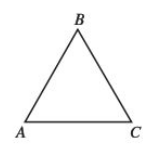
\includegraphics[width=4cm]{tequilatero} & 
	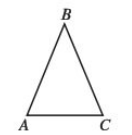
\includegraphics[width=4cm]{tisoceles}  & 
	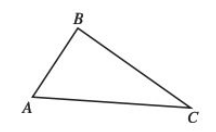
\includegraphics[width=4cm]{tescaleno} 
	\\ %\hline

	\textbf{Triángulo equilátero} & 
	\textbf{Triángulo isóceles} & 
	\textbf{Triángulo escaleno}                       
	\\ %\hline

	$\overline{AB} = \overline{AC} = \overline{BC}$ &
	$\overline{AB} = \overline{BC}$ &
	$\overline{AB} \ne \overline{AC} \ne \overline{BC}$ 
	\\

	\parbox{4cm}{
		\begin{center}
			Todos sus lados son iguales
		\end{center} 
	} & 
	\parbox{4cm}{
		\begin{center}
			Tiene 2 lados iguales
		\end{center} 
	} & 
	\parbox{4cm}{
		\begin{center}
			Todos sus lados son diferentes
		\end{center} 
	}                                 
\end{tabular}
% \end{adjustbox}
\end{figure*}

\subsubsection{Por sus ángulos}

\begin{figure*}[h!]
\def\arraystretch{1.5}%  1 is the default, change whatever you need
\caption[Clasificación de t]{Clasificación de triángulos. 
	Se toma como base la longitud de sus lados.
}
%TODO:- Corregir referencia de la tabla.
\labtab{clasiftriang}\label{clasiftriang}
\begin{tabular}{c  c  c }
	% \hline
  % TODO:- Corregir figuras
	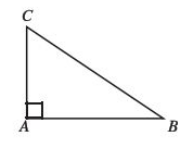
\includegraphics[width=4cm]{trectangulo} & 
	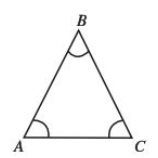
\includegraphics[width=4cm]{tacutangulo}  & 
	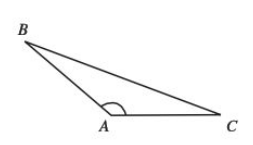
\includegraphics[width=4cm]{tobtusangulo} 
	\\ %\hline

	\textbf{Triángulo rectángulo} & 
	\textbf{Triángulo acutángulo} & 
	\textbf{Triángulo obtusángulo}                       
	\\ %\hline

	$\alpha = 90^\circ$ &
	$\alpha, \beta, \gamma < 90^\circ$ &
	$\alpha > 90^\circ$ 
	\\

	\parbox{4cm}{
		\begin{center}
			Tiene un ángulo recto
		\end{center} 
	} & 
	\parbox{4cm}{
		\begin{center}
			Sus 3 ángulos son agudos
		\end{center} 
	} & 
	\parbox{4cm}{
		\begin{center}
			Tiene un ángulo obtuso
		\end{center} 
	}                                 
\end{tabular}
% \end{adjustbox}
\end{figure*}

\newpage
\subsection{Rectas y puntos notables}

% TODO:- Recta de Euler

\begin{figure*}[h!]
\def\arraystretch{1.5}%  1 is the default, change whatever you need
\caption[Puntos notables]{Puntos notables y rectas en un triángulo}
%TODO:- Corregir referencia de la tabla.
\labtab{puntosnot}\label{puntosnot}
\begin{tabular}{c  c  c  c }
	\textbf{Altura} & 
	\textbf{Mediana} & 
	\textbf{Bisectriz} &
	\textbf{Mediatriz}
	\\
	\parbox{4cm}{ \begin{flushleft}
		Recta \textit{perpendicular} que va de un \textbf{vértice}
		al \textbf{lado opuesto}.
	\end{flushleft}}  & 
	\parbox{4cm}{ \begin{flushleft}
		Recta que va \textbf{vértice} con el \textbf{punto medio} 
		del lado opuesto. 
	\end{flushleft}}  & 
	\parbox{4cm}{ \begin{flushleft}		
		Recta que \textit{divide} a la \textit{mitad} a uno de los 	ángulos internos
		del triángulo. 
	\end{flushleft}}  & 		
	\parbox{4cm}{ \begin{flushleft}		
		Rectatextit{perpendicular} que pasa por el \textbf{punto medio}.
	\end{flushleft}}  
	\\
	\textbf{Ortocentro} & 
	\textbf{Baricentro} & 
	\textbf{Incentro} &
	\textbf{Circuncentro}
	\\
	\parbox{4cm}{ \begin{flushleft}
		Punto en donde se unen las \textbf{alturas}.
	\end{flushleft}}  & 
	\parbox{4cm}{ \begin{flushleft}
		Punto donde se intersectan las \textbf{medianas}.
	\end{flushleft}}  & 
	\parbox{4cm}{ \begin{flushleft}		
		Punto donde se intersectan las \textbf{bisectrices}.
	\end{flushleft}}  & 		
	\parbox{4cm}{ \begin{flushleft}		
		Punto donde se intersecan las \textbf{mediatrices}.
	\end{flushleft}}  
	\\
  % TODO:- Corregir figuras
	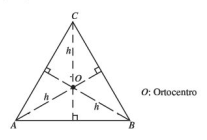
\includegraphics[width=4cm]{ortocentro} & 
	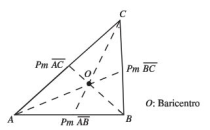
\includegraphics[width=4cm]{baricentro}  & 
	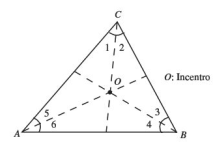
\includegraphics[width=4cm]{incentro} &
	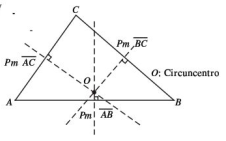
\includegraphics[width=4cm]{circuncentro} 
                                
\end{tabular}
% \end{adjustbox}
\end{figure*}

\subsection{Congruencia de triángulos}

2 triángulos son \textbf{congruentes}:
\marginnote{En pocas palabras, deben tener la misma forma y tamaño}
\begin{enumerate}[label=\alph*)]
	\item Sus \textit{lados} homólogos son iguales.
	\item Sus \textit{ángulos} homólogos son iguales.
\end{enumerate}

\marginnote{La notación para indicar congruencia es: $\cong$}

El concepto es muy sencillo, lo cierto es que en ``la vida real'' nunca nos
van a dar todas las medidas de un triángulo para poder comprobar que sus lados
y ángulos son homólogos, ¿Qué hacemos?\\

\textbf{\large3 casos}

\begin{figure*}[h!]
\def\arraystretch{1.5}%  1 is the default, change whatever you need
\caption[congruencia]{Casos de congruencia de triángulos. }
%TODO:- Corregir referencia de la tabla.
\labtab{congruencia}\label{congruencia}
\begin{tabular}{c  c  c }
	\textbf{Caso I} & 
	\textbf{Caso II} & 
	\textbf{Caso III}                       
	\\
	\textbf{Lados - Lado - Lado} & 
	\textbf{Ángulo - Lado - Ángulo} & 
	\textbf{Lado - Ángulo - Lado}                       
	\\
	$\begin{array} {lcl} 
		\overline{DE} & = & \overline{D'E'} \\ 
		\overline{EF} & = & \overline{E'F'} \\
		\overline{DF} & = & \overline{D'F'} 
	\end{array}$ &
	$\begin{array} {lcl} 
		H & = & H' \\ 
		\overline{HJ} & = & \overline{H'J'} \\
		J & = & J' 
	\end{array}$ &
	$\begin{array} {lcl} 
		\overline{KL} & = & \overline{K'L'} \\ 
		L & = & L' \\ 
		\overline{LM} & = & \overline{L'M'} 
	\end{array}$
	\\
  % TODO:- Corregir figuras
	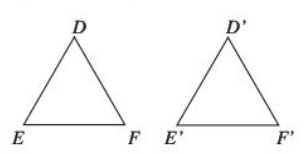
\includegraphics[width=4cm]{congruencia1} & 
	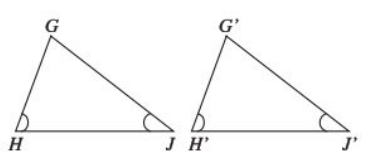
\includegraphics[width=4cm]{congruencia2}  & 
	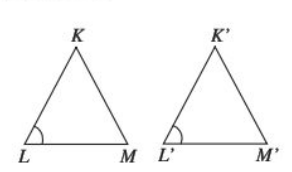
\includegraphics[width=4cm]{congruencia3} 
	
\end{tabular}
% \end{adjustbox}
\end{figure*}

\newpage
\subsection{Semejanza de triángulos}

2 triángulos son \textbf{semejantes} si:
\marginnote{Deben tener misma forma, pero diferente tamaño.}
\begin{enumerate}[label=\alph*)]
	\item Sus 3 \textit{ángulos} correspondientes son iguales.
	\item La \textit{proporción} de cada uno de sus 3 lados homólogos 
	\sidenote{Son aquellos cuyos águnos adyacentes son iguales} es proporcional.\\
		$$\dfrac{a}{a'} = \dfrac{b}{b'} = \dfrac{c}{c'}$$
\end{enumerate}

\textbf{\large3 casos}

\begin{figure*}[h!]
\def\arraystretch{1.5}%  1 is the default, change whatever you need
\caption[semejanza]{Casos de semejanza de triángulos. }
%TODO:- Corregir referencia de la tabla.
\labtab{semejanza}\label{semejanza}
\begin{tabular}{c  c  c }
	\textbf{Caso I} & 
	\textbf{Caso II} & 
	\textbf{Caso III}                       
	\\
	\textbf{2 ángulos homólogos} & 
	\textbf{3 Lados proporcionales} & 
	\parbox{5cm}{ \begin{center}
		\textbf{1 Ángulo igual y lados que forman dicho ángulos son proporcionales}                     
	\end{center}}  
	\\
	$\begin{array} {lcl} 
		C & = & C' \\ 
		A & = & A' 
	\end{array}$ &
	$\dfrac{a}{a'} = \dfrac{b}{b'} = \dfrac{c}{'c} $ &
	$\begin{array} {lcl} 
		K & = & K' \\ 
		\dfrac{g}{g'} &=& \dfrac{h}{h'}
	\end{array}$
	\\
  % TODO:- Corregir figuras
	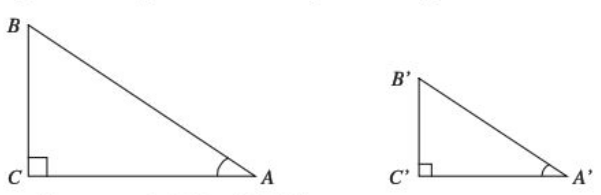
\includegraphics[width=5cm]{semejanza1} & 
	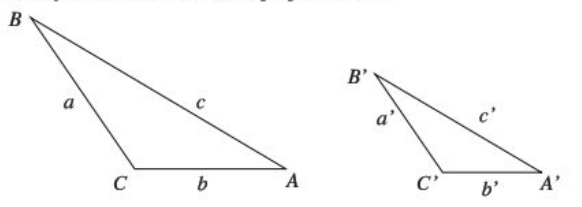
\includegraphics[width=5cm]{semejanza2}  & 
	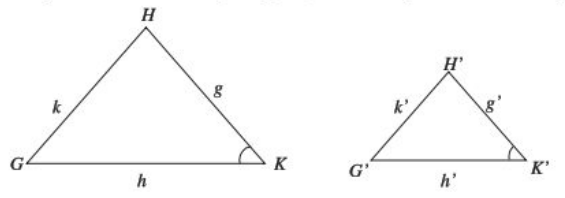
\includegraphics[width=5cm]{semejanza3} 
\end{tabular}
% \end{adjustbox}
\end{figure*}

% TODO:- Explicar proporciones.

\subsection{Teorema de Tales}

La consecuencia inmediata de la \textbf{semejanza del triángulos} es el
teorema conocido como \textbf{primer teorema de Tales}
\sidenote{A Tales de Mileto se le atribuyen dos teoremas con su nombre. 
El primero tiene que ver con la semejanza de triángulos y el segundo 
con triángulos inscritos en una circunferencia.}\\

El primer teorema de Tales dice que:\\

Si trazamos una recta paralela a uno de los lados de un triángulo se formará
otro que es semejante con el primero, como se observa en la figura 
\reffig{teorematales}.

\begin{figure}[ht!]
	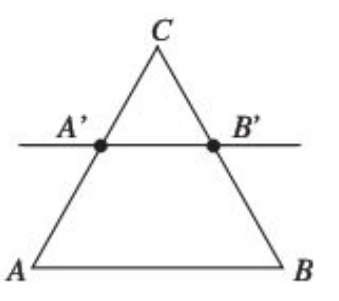
\includegraphics[width=5cm]{teorematales}
	\caption[teorematales]{Primer teorema de Tales.}
	\labfig{teorematales}
\end{figure}

Veamos un ejemplo:
% TODO:- Agregar ejemplo

% TODO:- Historia / Datos interesantes / Aplicaciones

\subsection{Teorema de Pitágoras}

El \textbf{teorema de Pitágoras} es uno de los teoremas que más aplicaciones 
tiene y del él han derivado muchos otros conceptos importantes de la 
trigonometría. 

\marginnote{A cada rato se emplea este concepto en física.}

El \textbf{teorema de Pitágoras} nos dice que:\\

Para cualquier \textit{triángulo rectángulo} el cuadrado de la hipotenusa
\sidenote{La hipotenusa es el lado más grande de un triángulo rectángulo.} es 
igual a la suma de los cuadrados de los catetos.\sidenote{Los catetos son los
lados que sobran después de definir quién es la hipotenusa.}

\begin{figure}[ht!]
	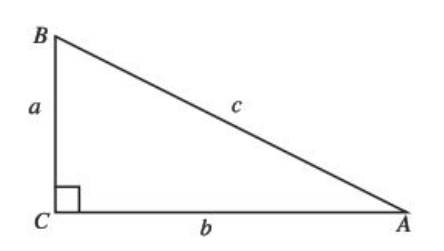
\includegraphics[width=5cm]{teoremapit}
	\caption[teoremapit]{Teorema de Pitágoras.}
	\labfig{teoremapit}
\end{figure}

En lenguaje matemático y con ayuda de la figura \reffig{teoremapit}, nos queda
como:

\[\boxed{c^2 = a^2 + b^2}\]

En donde: 
\begin{itemize}
	\item [\textbf{c}] es la \textit{hipotenusa} 
	\item [\textbf{a,b}] son los \textit{catetos}
\end{itemize}

Por medio del \textbf{teorema de Pitágoras} es posible clasificar o identificar
la naturalez de un triángulo, es decir, podemos decir si es \textit{acutángulo},
\textit{obtusángulo} o \textit{rectángulo}. 
\sidenote{Recuerda que el teorema de pitágoras se cumple (la igualdad) para 
triángulos rectángulos únicamente.}

\begin{enumerate}
	\item Si se cumple $c^2 = a^2 + b^2$, entonces hablamos de un triángulo 
		rectángulo.
	\item Si $c^2 \ne a^2 + b^2$ \sidenote[*]{Si la igualdad no se cumple}, 
		entonces puede que tengamos un triángulo \textit{acutángulo} o 
		\textit{obtusángulo}.
		\begin{itemize}
			\item Si $c^2 < a^2 + b^2$, entonce el triángulo es acutángulo.
			\item Si $c^2 > a^2 + b^2$, entonce el triángulo es obtusángulo.
		\end{itemize}
\end{enumerate}


\subsubsection{La semejanza en el triángulo rectángulo}

Dado un triángulo \textit{rectángulo}, a partir de la \textbf{hipotenusa} 
trazamos una \textbf{altura} hacia el vértice opuesto se formarán tres 
triángulos como muestra en la figura \reffig{semejrect}.

\begin{figure}[ht!]
	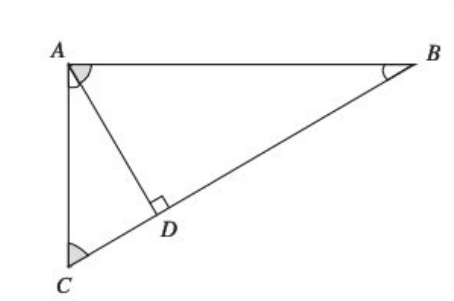
\includegraphics[width=5cm]{semejrect}
	\caption[semejrect]{Semejanza para triángulos rectángulos.}
	\labfig{semejrect}
\end{figure}

Los triángulos que se forman son semejantes de la siguiente manera

\begin{equation*}
\begin{array}{lcl}
	\widetriangle{ACD} & \sim & \widetriangle{BAD} \\
	\widetriangle{CAB} & \sim & \widetriangle{CDA} \\
	\widetriangle{CAB} & \sim & \widetriangle{ABD}
\end{array}
\end{equation*}

De lo anterior, puede demostrarse dos propiedades:

\begin{itemize}
	\setlength\itemsep{1.5em}
	\item $h^2 = \overline{CD}\cdot \overline{DB}$
	\item 
		$\begin{array}{lcl}
		\overline{AC} & = & \overline{CD} \cdot \overline{CB} \\
		\overline{AB} & = & \overline{CB} \cdot \overline{DB}
		\end{array}$
\end{itemize}


\subsection{Los ángulos (interiores) de un triángulo}

A continuación veremos las propiedades más importantes de los 
ángulos de un triángulo.

\begin{figure*}[h!]
\def\arraystretch{1.5}%  1 is the default, change whatever you need
\caption[propsTriangulos]{Propiedades elementales de los ángulos de los
	triángulos. 
}
%TODO:- Corregir referencia de la tabla.
\labtab{propstrig}\label{propstrig}
\begin{tabular}{c  c  c }
	\textbf{Propiedad I} & 
	\textbf{Propiedad II} & 
	\textbf{Propiedad III}                       
	\\
	\parbox{5cm}{ \begin{center}
		La suma de los ángulos interiores de un triángulo es igual a $180^\circ$	
	\end{center}}  &
	\parbox{5cm}{ \begin{center}
		La suma de los ángulos exteriores de un triángulo es igual a $360^\circ$
	\end{center}}  &
	\parbox{5cm}{ \begin{center}
		Un ángulo exterior es igual a la suma de los 2 interiores no adyacentes 
		a él
	\end{center}}  
	\\
  % TODO:- Corregir figuras
	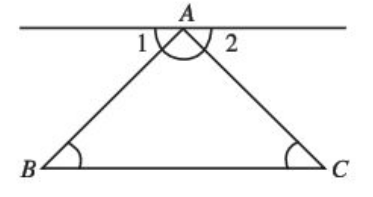
\includegraphics[width=5cm]{prop1} & 
	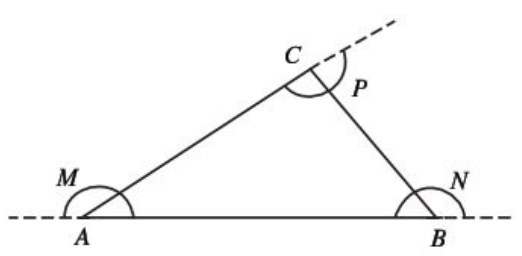
\includegraphics[width=5cm]{prop2}  & 
	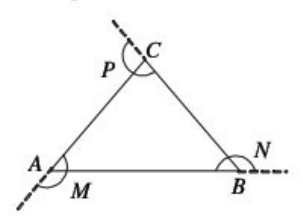
\includegraphics[width=5cm]{prop3} 
	\\ 
	$A + B + C = 180^\circ$ &
	$M + N + P = 360^\circ$&
	$\begin{array} {lcl} 
		M & = & B + C \\ 
		P & = & A + B \\ 
		N & = & A + C
	\end{array}$	
\end{tabular}
% \end{adjustbox}
\end{figure*}

\subsection{Razones trigonométricas}

Las razones trigonométricas son simplemente comparaciones de dos lados 
de un triángulo con respecto de un ángulo.

Primero, entendamos la terminología para nombrar cada uno de los lados de un 
triángulo.

% Insertar figura

\begin{itemize}
	\item \textbf{La hipotenusa} siempre es el lado más grande de un triángulo.
	\item \textbf{El cateto opuesto} se denomina así por que es el lado que está 
		en frente del ángulo de interés.
	\item \textbf{El cateto adyacente}, es el lado que está \textit{a un lado}
		del ángulo de interés.
\end{itemize}